\section{DOMÓTICA}

El término domótica proviene de la unión de las palabras \emph{domus} (que significa casa en latín) y \emph{tica} (de automática, palabra en griego). La Real Academa Española lo define como el <<conjunto de sistemas que automatizan las diferentes instalaciones de una vivienda>>.

En este proyecto se utilizará el concepto de domótica como la tecnología aplicada al Internet de las Cosas en el hogar, es decir, conectar nuestro hogar a la nube.

\subsection{Historia}

\parpic[r][]{
    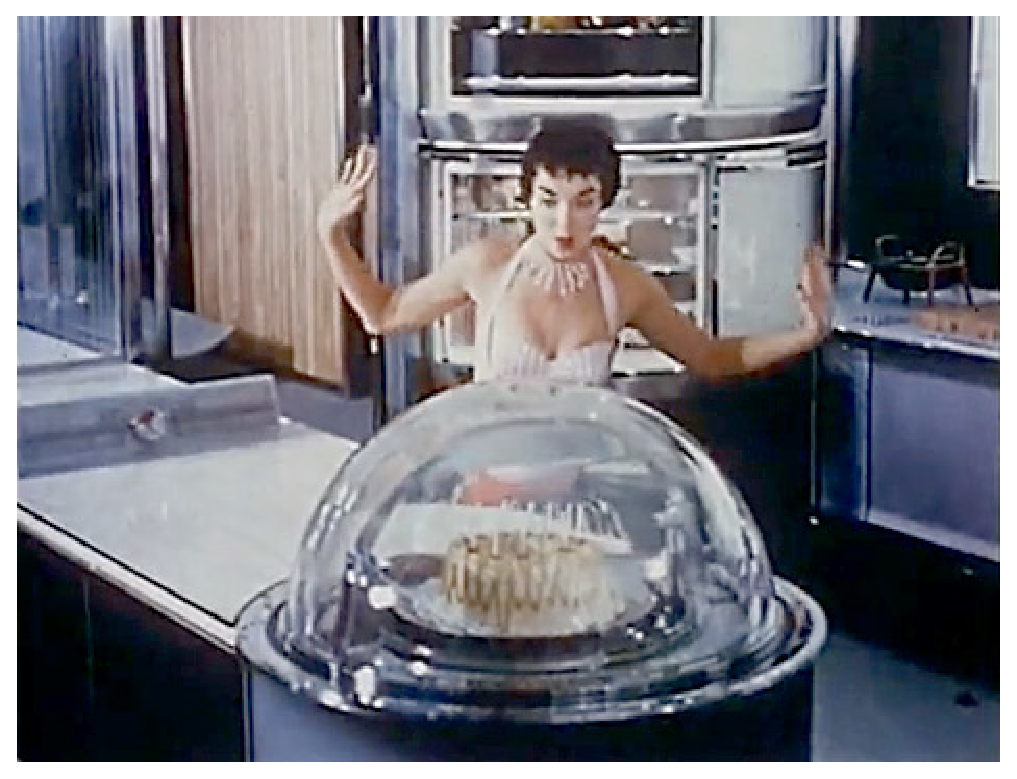
\includegraphics[keepaspectratio,width=0.25\textwidth]{Design_for_Dreaming_-_Cake_Under_Glass.eps}
    \label{fig:design-for-dreaming}
}

El hogar inteligente y automático comenzó a imaginarse en historias de ciencia ficción a inicios del siglo XX. En 1956 se emitió la película \emph{Design for Dreaming}~\ref{fig:design-for-dreaming} donde una mujer cae dormida y tiene una serie de sueños futuristas, incluyendo a \emph{Frigidaire}, la cocina automatizada del futuro.

